% FermiSets architecture figure.
% Compiles standalone: pdflatex fermisets_architecture.tex
% Thesis use: \includegraphics the resulting .pdf.
\documentclass[tikz,border=4pt]{standalone}
\usepackage{amsmath}
\usepackage{amssymb}
\usetikzlibrary{positioning, arrows.meta, matrix, backgrounds, calc}

% Okabe-Ito colorblind-safe palette: blue for the xi (symmetric) branch, orange
% for the eta (antisymmetric) branch. Everything else stays black/grey.
\definecolor{symblue}{RGB}{0,114,178}
\definecolor{antiorange}{RGB}{230,159,0}
\definecolor{inkgrey}{RGB}{60,60,60}

% fan-of-copies decoration behind an already-placed node NODE, tinted COLOR,
% indicating "one such vector per particle". Draw AFTER the node exists.
\newcommand{\fan}[2]{
  \begin{scope}[on background layer]
    \draw[thick, draw=#2!70, fill=#2!6]  ($(#1.south west)+(2.2mm,2.2mm)$) rectangle ($(#1.north east)+(2.2mm,2.2mm)$);
    \draw[thick, draw=#2!70, fill=#2!10] ($(#1.south west)+(1.1mm,1.1mm)$) rectangle ($(#1.north east)+(1.1mm,1.1mm)$);
  \end{scope}
}

\begin{document}
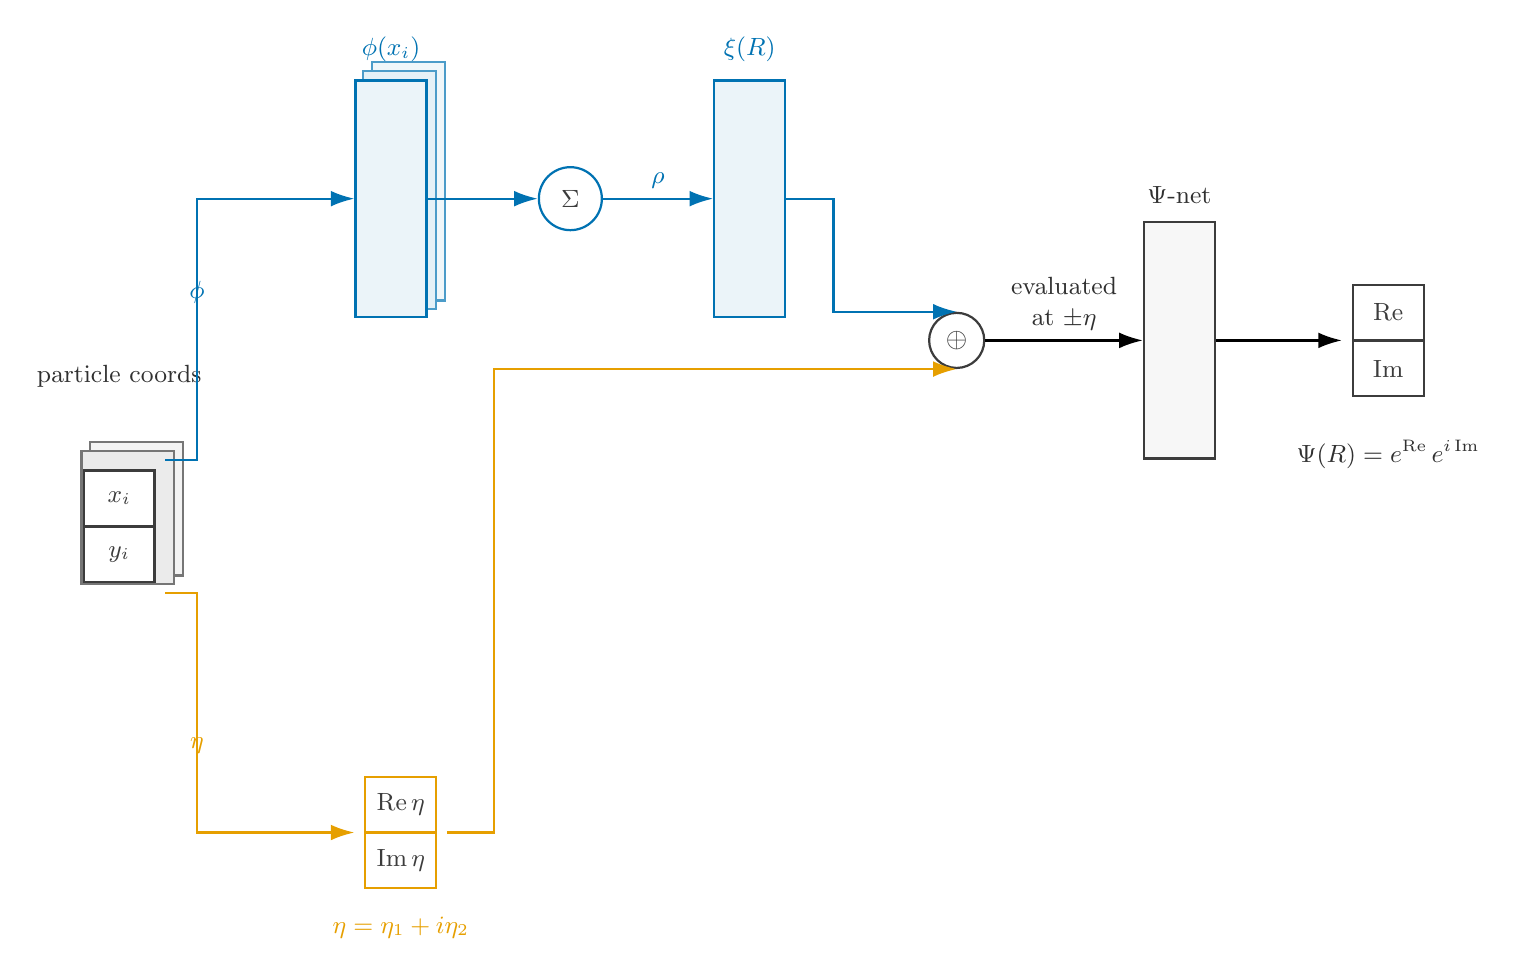
\begin{tikzpicture}[
    font=\normalsize,
    >={Latex[length=3mm,width=2mm]},
    every node/.style={text=inkgrey},
    cell/.style={draw=inkgrey, thick, minimum width=9mm, minimum height=7mm, inner sep=0pt, fill=white, font=\small},
    symcell/.style={cell, draw=symblue},
    anticell/.style={cell, draw=antiorange},
    vec2/.style={matrix of nodes, nodes={cell}, row sep=-\pgflinewidth, ampersand replacement=\&},
    vec2anti/.style={matrix of nodes, nodes={anticell}, row sep=-\pgflinewidth, ampersand replacement=\&},
    bar/.style={draw=inkgrey, thick, minimum width=9mm, minimum height=30mm, inner sep=0pt, fill=inkgrey!4},
    symbar/.style={bar, draw=symblue, fill=symblue!8},
    pool/.style={draw=symblue, thick, circle, minimum size=8mm, fill=white, font=\small},
    lbl/.style={font=\small, text=inkgrey!80!black},
    symlbl/.style={lbl, text=symblue},
    antilbl/.style={lbl, text=antiorange},
    arrow/.style={-{Latex[length=3mm,width=2mm]}, thick},
    symarrow/.style={arrow, symblue},
    antiarrow/.style={arrow, antiorange},
]

% ---------------------------------------------------------------- input ---
\matrix[vec2] (xin) {$x_i$ \\ $y_i$ \\};
\fan{xin}{inkgrey}
\node[lbl, above=8mm of xin] {particle coords};

% ------------------------------------------------------- xi branch (top) ---
\node[symbar, above right=18mm and 24mm of xin] (phi) {};
\fan{phi}{symblue}
\node[symlbl, above=1mm of phi] {$\phi(x_i)$};
\draw[symarrow] (xin.north east) -- ++(4mm,0) |- node[pos=0.28, above, symlbl] {$\phi$} (phi.west);

\node[pool, right=14mm of phi] (sum) {$\Sigma$};
\draw[symarrow] (phi) -- (sum);

\node[symbar, right=14mm of sum] (xi) {};
\node[symlbl, above=1mm of xi] {$\xi(R)$};
\draw[symarrow] (sum) -- node[above, symlbl] {$\rho$} (xi);

% --------------------------------------------------- eta branch (bottom) ---
\matrix[vec2anti, below right=22mm and 24mm of xin] (eta) {$\mathrm{Re}\,\eta$ \\ $\mathrm{Im}\,\eta$ \\};
\draw[antiarrow] (xin.south east) -- ++(4mm,0) |- node[pos=0.28, below, antilbl] {$\eta$} (eta.west);
\node[antilbl, below=1mm of eta] {$\eta = \eta_1 + i\eta_2$};

% ---------------------------------------------------------- concatenate ---
\node[draw=inkgrey, thick, circle, minimum size=7mm, right=18mm of xi, yshift=-18mm, inner sep=0pt] (concat) {$\oplus$};
\draw[symarrow] (xi.east) -- ++(6mm,0) |- (concat.north);
\draw[antiarrow] (eta.east) -- ++(6mm,0) |- (concat.south);

% ---------------------------------------------------------- big Psi net ---
\node[bar, right=20mm of concat] (bignet) {};
\node[lbl, above=1mm of bignet] {$\Psi$-net};
\draw[arrow] (concat) -- node[above, lbl, text width=22mm, align=center, pos=0.5] {evaluated at $\pm\eta$} (bignet);

\matrix[vec2, right=16mm of bignet] (out) {$\mathrm{Re}$ \\ $\mathrm{Im}$ \\};
\draw[arrow] (bignet) -- (out);
\node[lbl, below=3mm of out, align=center] {$\Psi(R) = e^{\mathrm{Re}}\, e^{i\,\mathrm{Im}}$};

\end{tikzpicture}
\end{document}
